\documentclass[12pt]{article}

\usepackage{sbc-template}
\usepackage{graphicx,url}
\usepackage[utf8]{inputenc}
% \usepackage[brazil]{babel}
\usepackage{tikz} %Ferramenta mais complexa e poderosa para criar elementos gráficos
\usetikzlibrary{calc}
\usepackage{tkz-fct,tkz-euclide,tkz-base,tikz}
\tikzset{bolinha/.style={circle, draw, fill=none,
		inner sep=1pt, minimum width=1pt}}
\tikzset{bola/.append style={circle, draw, fill=none,
		inner sep=2pt, minimum width=1pt, fill=gray!50}}

\usepackage{colortbl}
\usepackage{booktabs}
\usepackage{hhline}
\usepackage{array}
\usepackage{color}
\usepackage{outlines}
\usepackage{dsfont}
\usepackage{amsmath}
\usepackage{breakcites}
\renewcommand{\qedsymbol}{$\blacksquare$}

\usepackage{amsmath,amssymb,amsthm}
\tikzset{
	square/.style={%
		draw=none,
		circle,
		append after command={%
			\pgfextra \draw[black] (\tikzlastnode.north-|\tikzlastnode.west) rectangle 
			(\tikzlastnode.south-|\tikzlastnode.east);\endpgfextra}
	}
}

%Interface para algoritmos%
%%%%%%%%%%%%%%%%%%%%%%%%%%%%%%%%%%%%%%%
\usepackage{algorithm}
\usepackage{algpseudocode}
% \algsetup{linenosize=\small}
%%%%%%%%%%%%%%%%%%%%%%%%%%%%%%%%%%%%%%%%%%%%%%%%%%
\usepackage{hyperref}
\hypersetup{
	colorlinks=true,
	linkcolor=blue,
	filecolor=blue,      
	urlcolor=blue,
	citecolor=black,
	% pdftitle={Overleaf Example},
	% pdfpagemode=FullScreen,
}
\urlstyle{same}
%\sloppy


\title{Using Markov chains and Monte Carlo simulations to solve Minimum Diameter Spanning Tree Problem}

\author{Amanda Ferreira de Azevedo\inst{1}, Wanderson Douglas Lomenha Pereira\inst{1}\\
\url{https://github.com/afazevedo/project_mcmc}}


\address{
	Universidade Federal do Rio de Janeiro\\
	Instituto Alberto Luiz Coimbra de Pós-Graduação e Pesquisa em Engenharia\\
	Programa de Engenharia de Sistemas e Computação
	\email{\{afazevedo,wlomenha\}@cos.ufrj.br}
}

\begin{document} 

\maketitle
                                                          
\begin{abstract}
        Given an undirected graph G=(V, E), we investigate the Budget Minimum Diameter Spanning Tree Problem, seeking the minimum diameter spanning tree of $G$. The diameter is given by the number of edges in the most extensive path of a tree. Moreover, costs are associated with all the edges of $G$, and the sum of the edge costs of this tree may not exceed a given budget value. Thus, feasible trees must necessarily be spanning. Barely investigated in the literature, these problems have much application, mainly in the telecommunications area. Furthermore, in the literature it has been proven to be an NP-Hard problem. Our approach uses the simulated annealing algorithm that solves the problem through a Markov chain simulation. This chain induces a lazy random walk between spanning trees, and the probability transition to each neighbor is uniformly equal. The results show good approximations when compared to the optimal solution. Thus, to our knowledge, is the first use of random heuristics algorithms proposed for this problem. Therefore, we show that the chain takes many transitions to converge, and the algorithm performance is related to the sparseness of G.
\end{abstract}
%     
%\begin{resumo} 
%  Este meta-artigo descreve o estilo a ser usado na confecção de artigos e
%  resumos de artigos para publicação nos anais das conferências organizadas
%  pela SBC. É solicitada a escrita de resumo e abstract apenas para os artigos
%  escritos em português. Artigos em inglês deverão apresentar apenas abstract.
%  Nos dois casos, o autor deve tomar cuidado para que o resumo (e o abstract)
%  não ultrapassem 10 linhas cada, sendo que ambos devem estar na primeira
%  página do artigo.
%\end{resumo}

\section{Problem definition and literature survey}

 Let $G = (V, E)$ be a finite undirected connected graph with a set $V$ of vertices and a set $E$ of edges. Assume that a cost $c_{e}$ is associated to each edge $e = \{i, j\} \in E$. A \emph{tree} $T = (V_T, E_T)$, with $ V_T \subseteq V $ and $E_T \subseteq E$, is a connected and acyclic subgraph of $G$. A \emph{spanning tree} is a tree that contains all the vertices of the graph, i.e., when $V_T = V$. Among all the spanning trees of $G$, the one with the lowest cost is the optimal solution to the \emph{Minimum Spanning Tree Problem} (MST).

A \emph{path} in $G$ is called \emph{simple} when it does not visit the same node more than once. Denote by $d_{ij}$ the length of the shortest simple path connecting the vertices $i,j \in V$, i.e., the \emph{distance} between them. Finally, the largest distance between any pair of nodes in $G$ is called the \emph{diameter} of $G$. Let $B$ be an upper limit for the total cost of a given tree edges. Thus, the \emph{Budget Minimum Diameter Spanning Tree Problem} (BDSTP) aims to find a spanning tree $T$ with minimum diameter, where $\sum_{e\in E} c_e \leq B$. 

BMDSTP was introduced by \cite{Plesnik1981}, who proved to be an NP-Hard problem. As far as we know, there are no non-exact algorithms that solve it in the literature. The first exact algorithms, however, were proposed this year by \cite{Amanda2021}. When all the costs $c_e$ are all equal to $1$ and $B = |V|-1$, the problem is equivalent to \emph{1-center problem} (see \cite{Hakimi1978} for details). Thus, 
under these conditions exists a polynomial-time algorithm that solves it despite the instance size. Therefore, the budget constraint becomes redundant, and the problem could just be named \emph{Minimum Diameter Spanning Tree Problem} (MDSTP). For example, consider the graph of the states of Brazil shown in Figure~\ref{fig:statesbrazil}.


\begin{figure}[H]
	\begin{center}
		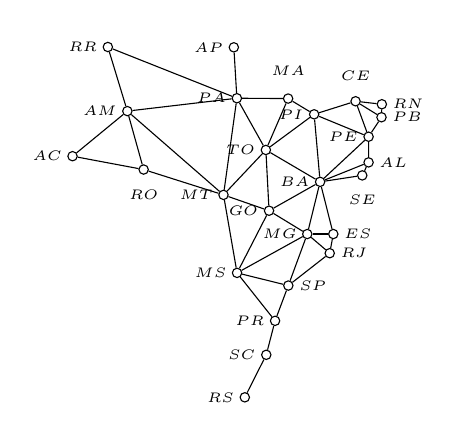
\begin{tikzpicture}
		[scale=0.9,auto=left]   
			\tikzstyle{every node}=[circle, draw, fill=white,
		inner sep=1.2pt, minimum width=1.2pt]
		%-----A
		 \node[label=left: \tiny{$RS$}]  (RS) at (3.51771,0.71697) {};
		 \node[label=left: \tiny{$SC$}]  (SC) at (3.82081,1.31696) {};
		 \node[label=left: \tiny{$PR$}]  (PR) at (3.9449,1.79661) {};
		 \node[label=right: \tiny{$SP$}]  (SP) at (4.1317,2.29403) {};
		 \node[label=left: \tiny{$MS$}]  (MS) at (3.40845,2.4728) {};
		 \node[label=right: \tiny{$RJ$}]  (RJ) at (4.71611,2.75066) {};
		 \node[label=right: \tiny{$ES$}]  (ES) at (4.76642,3.02098) {};
		 \node[label=left: \tiny{$MG$}]  (MG) at (4.39932,3.02098) {};
		 \node[label=left: \tiny{$GO$}]  (GO) at (3.85982,3.35025) {};
		 \node[label=left: \tiny{$MT$}]  (MT) at (3.21712,3.57363) {};
		 \node[label=left: \tiny{$BA$}]  (BA) at (4.58039,3.75741) {};
		 \node[label=below: \tiny{$SE$}]  (SE) at (5.17517,3.84839) {};
		 \node[label=right: \tiny{$AL$}]  (AL) at (5.26448,4.03205) {};
		 \node[label=left: \tiny{$PE$}]  (PE) at (5.26448,4.39432) {};
		 \node[label=right: \tiny{$PB$}]  (PB) at (5.44645,4.66896) {};
		 \node[label=right: \tiny{$RN$}]  (RN) at (5.45151,4.85262) {};
		 \node[label=above: \tiny{$CE$}]  (CE) at (5.08082,4.89474) {};
		 \node[label=left: \tiny{$PI$}]  (PI) at (4.49622,4.71063) {};
		 \node[label=above: \tiny{$MA$}]  (MA) at (4.12919,4.93268) {};
		 \node[label=left: \tiny{$TO$}]  (TO) at (3.81491,4.20743) {};
		 \node[label=left: \tiny{$PA$}]  (PA) at (3.40601,4.93749) {};
		 \node[label=left: \tiny{$AP$}]  (AP) at (3.36296,5.65585) {};
		 \node[label=left: \tiny{$RR$}]  (RR) at (1.58515,5.66035) {};
		 \node[label=left: \tiny{$AM$}]  (AM) at (1.86035,4.75576) {};
		 \node[label=left: \tiny{$AC$}]  (AC) at (1.08682,4.11959) {};
		 \node[label=below: \tiny{$RO$}]  (RO) at (2.09036,3.93125) {};
		 
		 
		 \foreach \from/\to in {RS/SC,SC/PR,PR/SP,PR/MS,SP/RJ,SP/MG,SP/MS,RJ/ES,RJ/MG,MS/MG,ES/MG,ES/BA,MG/BA,MG/GO,MS/GO,MS/MT,GO/BA,GO/TO,GO/MT,TO/BA,TO/PI,TO/MA,TO/PA,TO/MT,MT/PA,PA/MA,MA/PI,PI/BA,PI/CE,PI/PE,PE/BA,BA/AL,BA/SE,SE/AL,AL/PE,PE/PB,PE/CE,CE/PB,CE/RN,RN/PB,AP/PA,RR/PA,RR/AM,AM/PA,AM/MT,RO/MT,RO/AM,AC/RO,AC/AM}  
		 \draw (\from) -- (\to); 
		 
		 
		\end{tikzpicture}   
    \end{center}
    \caption{Graph of the states of Brazil}
      \label{fig:statesbrazil}
	\end{figure}


An illustration of a comparison between the optimal spanning tree of MDSTP, MST, and BMDSTP is given in Figure~\ref{fig:compst}.


\begin{figure}[H]
	\begin{center}
		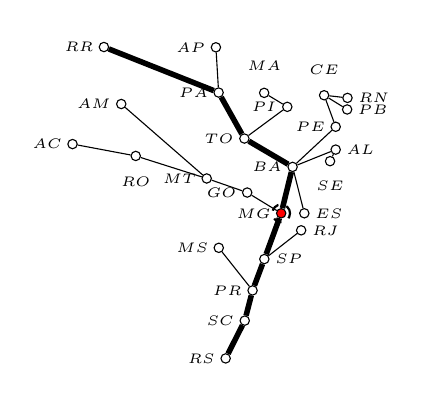
\begin{tikzpicture}
		[scale=0.8,auto=left]   
			\tikzstyle{every node}=[circle, draw, fill=white,
		inner sep=1.2pt, minimum width=1.2pt]
		%-----A
		 \node[label=left: \tiny{$RS$}]  (RS) at (3.51771,0.71697) {};
		 \node[label=left: \tiny{$SC$}]  (SC) at (3.82081,1.31696) {};
		 \node[label=left: \tiny{$PR$}]  (PR) at (3.9449,1.79661) {};
		 \node[label=right: \tiny{$SP$}]  (SP) at (4.1317,2.29403) {};
		 \node[label=left: \tiny{$MS$}]  (MS) at (3.40845,2.4728) {};
		 \node[label=right: \tiny{$RJ$}]  (RJ) at (4.71611,2.75066) {};
		 \node[label=right: \tiny{$ES$}]  (ES) at (4.76642,3.02098) {};
		 \node[label=left: \tiny{$MG$}, fill = red]  (MG) at (4.39932,3.02098) {};
		 \node[label=left: \tiny{$GO$}]  (GO) at (3.85982,3.35025) {};
		 \node[label=left: \tiny{$MT$}]  (MT) at (3.21712,3.57363) {};
		 \node[label=left: \tiny{$BA$}]  (BA) at (4.58039,3.75741) {};
		 \node[label=below: \tiny{$SE$}]  (SE) at (5.17517,3.84839) {};
		 \node[label=right: \tiny{$AL$}]  (AL) at (5.26448,4.03205) {};
		 \node[label=left: \tiny{$PE$}]  (PE) at (5.26448,4.39432) {};
		 \node[label=right: \tiny{$PB$}]  (PB) at (5.44645,4.66896) {};
		 \node[label=right: \tiny{$RN$}]  (RN) at (5.45151,4.85262) {};
		 \node[label=above: \tiny{$CE$}]  (CE) at (5.08082,4.89474) {};
		 \node[label=left: \tiny{$PI$}]  (PI) at (4.49622,4.71063) {};
		 \node[label=above: \tiny{$MA$}]  (MA) at (4.12919,4.93268) {};
		 \node[label=left: \tiny{$TO$}]  (TO) at (3.81491,4.20743) {};
		 \node[label=left: \tiny{$PA$}]  (PA) at (3.40601,4.93749) {};
		 \node[label=left: \tiny{$AP$}]  (AP) at (3.36296,5.65585) {};
		 \node[label=left: \tiny{$RR$}]  (RR) at (1.58515,5.66035) {};
		 \node[label=left: \tiny{$AM$}]  (AM) at (1.86035,4.75576) {};
		 \node[label=left: \tiny{$AC$}]  (AC) at (1.08682,4.11959) {};
		 \node[label=below: \tiny{$RO$}]  (RO) at (2.09036,3.93125) {};
		 
		  \draw[thick,dashed] (4.39932,3.02098) circle (0.14cm); 
		 
		  \draw[line width = 2] (RR) -- (PA);
		  \draw[line width = 2] (PA) -- (TO);
		  \draw[line width = 2] (TO) -- (BA);
		  \draw[line width = 2] (BA) -- (MG);
		  \draw[line width = 2] (MG) -- (SP);
		  \draw[line width = 2] (SP) -- (PR);
		  \draw[line width = 2] (PR) -- (SC);
		  \draw[line width = 2] (SC) -- (RS);
		  
		 
		 \foreach \from/\to in {RR/PA, AP/PA, PA/TO, TO/PI, PI/MA, TO/BA, BA/AL, AL/SE, BA/ES, BA/PE, PE/CE, CE/RN, CE/PB, BA/MG, MG/GO, GO/MT, MT/AM, MT/RO, RO/AC,SP/MG, SP/RJ, SP/PR, PR/MS, PR/SC, SC/RS}  
		 \draw (\from) -- (\to); 
		 
		 
		\end{tikzpicture} 
    \hspace{0.01cm}
        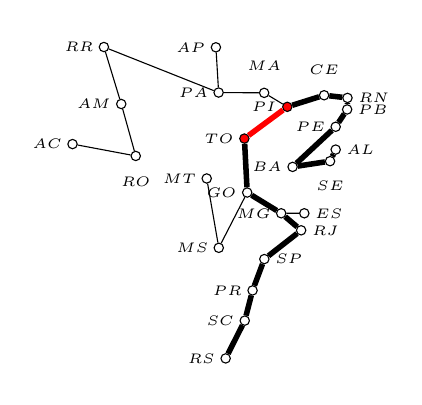
\begin{tikzpicture}
        [scale=0.8,auto=left]
            \tikzstyle{every node}=[circle, draw, fill=white,
        inner sep=1.2pt, minimum width=1.2pt]
        %-----A
         \node[label=left: \tiny{$RS$}]  (RS) at (3.51771,0.71697) {};
         \node[label=left: \tiny{$SC$}]  (SC) at (3.82081,1.31696) {};
         \node[label=left: \tiny{$PR$}]  (PR) at (3.9449,1.79661) {};
         \node[label=right: \tiny{$SP$}]  (SP) at (4.1317,2.29403) {};
         \node[label=left: \tiny{$MS$}]  (MS) at (3.40845,2.4728) {};
         \node[label=right: \tiny{$RJ$}]  (RJ) at (4.71611,2.75066) {};
         \node[label=right: \tiny{$ES$}]  (ES) at (4.76642,3.02098) {};
         \node[label=left: \tiny{$MG$}]  (MG) at (4.39932,3.02098) {};
         \node[label=left: \tiny{$GO$}]  (GO) at (3.85982,3.35025) {};
         \node[label=left: \tiny{$MT$}]  (MT) at (3.21712,3.57363) {};
         \node[label=left: \tiny{$BA$}]  (BA) at (4.58039,3.75741) {};
         \node[label=below: \tiny{$SE$}]  (SE) at (5.17517,3.84839) {};
         \node[label=right: \tiny{$AL$}]  (AL) at (5.26448,4.03205) {};
         \node[label=left: \tiny{$PE$}]  (PE) at (5.26448,4.39432) {};
        \node[label=right: \tiny{$PB$}]  (PB) at (5.44645,4.66896) {};
         \node[label=right: \tiny{$RN$}]  (RN) at (5.45151,4.85262) {};
         \node[label=above: \tiny{$CE$}]  (CE) at (5.08082,4.89474) {};
         \node[label=left: \tiny{$PI$}, fill = red]  (PI) at (4.49622,4.71063) {};
         \node[label=above: \tiny{$MA$}]  (MA) at (4.12919,4.93268) {};
         \node[label=left: \tiny{$TO$}, fill = red]  (TO) at (3.81491,4.20743) {};
         \node[label=left: \tiny{$PA$}]  (PA) at (3.40601,4.93749) {};
         \node[label=left: \tiny{$AP$}]  (AP) at (3.36296,5.65585) {};
         \node[label=left: \tiny{$RR$}]  (RR) at (1.58515,5.66035) {};
         \node[label=left: \tiny{$AM$}]  (AM) at (1.86035,4.75576) {};
         \node[label=left: \tiny{$AC$}]  (AC) at (1.08682,4.11959) {};
         \node[label=below: \tiny{$RO$}]  (RO) at (2.09036,3.93125) {};

          \draw[line width = 2] (AL) -- (SE);
          \draw[line width = 2] (SE) -- (BA);
          \draw[line width = 2] (BA) -- (PE);
          \draw[line width = 2] (PE) -- (PB);
          \draw[line width = 2] (PB) -- (RN);
          \draw[line width = 2] (RN) -- (CE);
          \draw[line width = 2] (CE) -- (PI);
          \draw[line width = 2, color = red] (PI) -- (TO);
          \draw[line width = 2] (TO) -- (GO);
          \draw[line width = 2] (MG) -- (GO);
          \draw[line width = 2] (MG) -- (RJ);
          \draw[line width = 2] (RJ) -- (SP);
          \draw[line width = 2] (SP) -- (PR);
          \draw[line width = 2] (PR) -- (SC);
          \draw[line width = 2] (SC) -- (RS);

         \foreach \from/\to in {RS/SC, SC/PR, PR/SP, SP/RJ, RJ/MG, MG/ES, MG/GO, GO/MS, MS/MT, GO/TO, PI/CE, CE/RN, RN/PB, PB/PE, PE/BA, BA/SE, SE/AL, PI/MA, MA/PA, PA/AP, PA/RR, RR/AM, AM/RO, RO/AC}
         \draw (\from) -- (\to); 


        \end{tikzpicture}
        \hspace{0.1cm}
        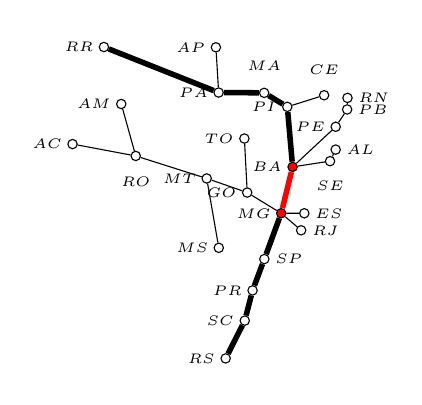
\begin{tikzpicture}
        [scale=0.8,auto=left]
            \tikzstyle{every node}=[circle, draw, fill=white,
        inner sep=1.2pt, minimum width=1.2pt]
        %-----A
         \node[label=left: \tiny{$RS$}]  (RS) at (3.51771,0.71697) {};
         \node[label=left: \tiny{$SC$}]  (SC) at (3.82081,1.31696) {};
         \node[label=left: \tiny{$PR$}]  (PR) at (3.9449,1.79661) {};
         \node[label=right: \tiny{$SP$}]  (SP) at (4.1317,2.29403) {};
         \node[label=left: \tiny{$MS$}]  (MS) at (3.40845,2.4728) {};
         \node[label=right: \tiny{$RJ$}]  (RJ) at (4.71611,2.75066) {};
         \node[label=right: \tiny{$ES$}]  (ES) at (4.76642,3.02098) {};
         \node[label=left: \tiny{$MG$}, fill = red]  (MG) at (4.39932,3.02098) {};
         \node[label=left: \tiny{$GO$}]  (GO) at (3.85982,3.35025) {};
         \node[label=left: \tiny{$MT$}]  (MT) at (3.21712,3.57363) {};
         \node[label=left: \tiny{$BA$}, fill = red]  (BA) at (4.58039,3.75741) {};
         \node[label=below: \tiny{$SE$}]  (SE) at (5.17517,3.84839) {};
         \node[label=right: \tiny{$AL$}]  (AL) at (5.26448,4.03205) {};
         \node[label=left: \tiny{$PE$}]  (PE) at (5.26448,4.39432) {};
         \node[label=right: \tiny{$PB$}]  (PB) at (5.44645,4.66896) {};
         \node[label=right: \tiny{$RN$}]  (RN) at (5.45151,4.85262) {};
         \node[label=above: \tiny{$CE$}]  (CE) at (5.08082,4.89474) {};
         \node[label=left: \tiny{$PI$}]  (PI) at (4.49622,4.71063) {};
         \node[label=above: \tiny{$MA$}]  (MA) at (4.12919,4.93268) {};
         \node[label=left: \tiny{$TO$}]  (TO) at (3.81491,4.20743) {};
         \node[label=left: \tiny{$PA$}]  (PA) at (3.40601,4.93749) {};
         \node[label=left: \tiny{$AP$}]  (AP) at (3.36296,5.65585) {};
         \node[label=left: \tiny{$RR$}]  (RR) at (1.58515,5.66035) {};
         \node[label=left: \tiny{$AM$}]  (AM) at (1.86035,4.75576) {};
         \node[label=left: \tiny{$AC$}]  (AC) at (1.08682,4.11959) {};
         \node[label=below: \tiny{$RO$}]  (RO) at (2.09036,3.93125) {};
         
         %\draw[thick,dashed] (4.489855,3.389195) circle (0.55cm); 
         
         
         \draw[line width = 2] (RR) -- (PA);
         \draw[line width = 2] (PA) -- (MA);
         \draw[line width = 2] (MA) -- (PI);
         \draw[line width = 2] (PI) -- (BA);
         \draw[line width = 2, color = red] (BA) -- (MG);
         \draw[line width = 2] (MG) -- (SP);
         \draw[line width = 2] (SP) -- (PR);
         \draw[line width = 2] (PR) -- (SC);
         \draw[line width = 2] (SC) -- (RS);
         
    
         \foreach \from/\to in {RN/PB, PB/PE, PE/BA, BA/SE, SE/AL, PI/CE, PA/AP, MG/RJ, MG/ES, MG/GO, GO/TO, GO/MT, MT/MS, MT/RO, RO/AM, RO/AC}
         \draw (\from) -- (\to); 

    % custo menor do que $B= 12733$
        \end{tikzpicture}
      \end{center}
      \caption{Comparison between the optimal spanning tree of MDSTP, MST, and BMDSTP respectively}
      \label{fig:compst}
    \end{figure}

%%%%fotinha do estados comparando os três

% \begin{figure}[H]

% \end{figure}


\section{Methodology}


The \emph{simulated annealing algorithm} is a meta-heuristic founded in the model of \cite{Metropolis1953}, which was adapted in the computational context by \cite{Kirkpatrick1983, Cern1985}. Moreover, is a \emph{Monte Carlo} technique inspired by an analogy with annealing, a physical phenomenon of thermodynamics. \emph{Annealing} consists of raising the temperature of the metal by injecting energy into the structure and then slowly cooling the metal. Thus, the general idea of the algorithm is to solve a minimization problem in analogy to this heating and cooling scheme. 

To decide whether a given movement is accepted or not, a probabilistic process controlled by \cite{Hastings1970} technique is used. One of the essential parameters for this process is the temperature, which controls the balance between intensification and diversification of the algorithm. When a new randomly generated solution has a cost worse than the current solution, the solution is accepted by a simplification of the probability distribution proposed by Maxwell-Boltzmann, and later simplified by Metropolis-Hastings \cite{Maxwell1860}. Thus, the probability of an energy variation $\Delta(s)$ of a transition between configurations in this distribution is given by:

\begin{equation}
    P(\Delta(s)) = e^{-\frac{\Delta(s)}{T}}
    \label{eq}
\end{equation}

If we are in a minimization problem, when $\Delta(s) < 0$, accepts with probability 1 uniformly between neighbors better than $s$. Additionally, when $\Delta(s) > 0$, accept with probability given by equation \ref{eq}. Therefore, when $\Delta = 0$, the acceptance is indifferent, since there is no change.


\subsection{Simulated Annealing and Markov Chains}

Let $S$ be a finite set of states in a Markov Chain with a function $f: S \rightarrow \mathds{R}$ associated to them. Formally, the general optimization problem in this context aim to find a state $s \in S$ that minimizes $f(s)$. Intuitively, let us take the inverse of $f$ as the stationary distribution of this chain and only accept states that provides improvement. In a sufficiently long time, we are likely to end up in a state $s$ where $f(s)$ is minimum. Using this strategy, however, we can end up at a local minimum. Then, if we control this "greed" with randomness and gradually increase it, we can highly get closer to the optimal solution. Hence, if we create a \textit{family of Markov chains}, each of which with an increasingly greedy stationary distribution, we can get even more close to the optimum. Thus, we will use the so-called \emph{Boltzmann} distribution to deal with this phenomenon, using the cooling idea seen in the last section. Therefore, we will create a Markov chain using Boltzmann distribution as its stationary distribution, as follows:

$$\pi_s = \frac{e^{\frac{-f(s)}{T}}}{\sum_{s \in S}e^{\frac{-f(s)}{T}}}$$

For a fixed and non-negative $T$, the smaller $f(s)$, the greater the stationary distribution. Thus, smaller values of $f(s)$ have exponentially larger probability. 
The guarantee that in a certain number of steps this chain will converge to the optimal solution is given by the following theorem:\\

\noindent\textbf{Theorem:} Let $S$ be a finite set and let $f: S \rightarrow \mathds{R}$ be arbitrary. For $T>0$, let $\alpha(T)$ denote the probability that a random element $s'$ chosen according to the \emph{Boltzmann} distribution $\pi_s$ satisfies: $f(s') = \displaystyle min_{s\in S} f(s)$ then $\displaystyle \lim_{T \rightarrow 0} \alpha(T) = 1$. Proof: See \cite{Olle2002}.

Hence, the Markov chain using $\pi_s$ as a stationary distribution and decreasing $T$,  increases the chances of choosing a minimum. The choice of how many iterations on each temperature should be done is called the annealing schedule, and their choice is crucial since we know that converges ‘‘sufficiently slowly". As \cite{Olle2002} said, \emph{‘‘The choice of annealing schedule in practice is therefore a highly delicate balance: On one hand, we want it to be fast enough to get convergence in reasonable time, and on the other hand, we want it to be slow enough to avoid converging to an element which is not an $f$-minimizer."}


\subsection{Our work}

Let $S = \{s_1,s_2, \dots\}$ be a state space. Every state $s_i \in S$ is a spanning tree of a given graph $G = (V,E)$. The other main ingredients are two functions, which we call the \emph{diameter function} and \emph{cost function}. The diameter function, $f: S \rightarrow \mathds{Z}$, is a function from the state space $S$ to any integer value in $\mathds{Z}$, which we use to calculate the diameter of given tree. Moreover, the cost function $g: S \rightarrow \mathds{R}$ is a function from the state space $S$ to any real value, which we use to calculate the total cost of a given tree. The transitions between any spanning trees is given by the algorithm named as \emph{cycle transition}, described below:
\vspace{0.3cm}
\begin{enumerate}
    \item Uniformly choose an edge in $E(G) - E(T)$ where $T$ is the current tree;
    \item Uniformly choose an edge in the cycle and remove;
    \item Return $T$.
\end{enumerate}
\vspace{0.3cm}

Consequently, the number of possible neighbors of each state is given by $|C|\cdot(m-n+1)$, where $|C|$ is the size of the imposed cycle, and $n,m$ is the number of nodes and edges, respectively. If the chosen edge was the same added edge, we stay in the same position, inducing a self-loop. Moreover, if $G$ is a complete graph with $n$ vertices, the total number of spanning trees is $n^{(n-2)}$, namely \emph{Cayley's} formula. Otherwise, if $G$ is not a complete graph, the number of spanning trees can be calculated by \emph{ Kirchhoff's Theorem}. For example, applying to the graph of the states of Brazil given as an example, the total number of states in our chain would be 5310501721.   

To generate an initial solution for the chain, we use an algorithm proposed by \cite{broder1989generating}, named \textbf{generate}, described as follows:
\vspace{0.3cm}
\begin{enumerate}
    \item Simulate a random walk in $G$ starting at $s$ until every node is visited, storing the first visit to each node.
    \item To each node $i \in V-s$, we take the edge $\{j,i\}$ and we add to the tree, $T$, where $j$ corresponds the first visit to $i$.
    \item Return $T$
\end{enumerate}
\vspace{0.3cm}
The algorithm complexity is $O(n\log{n})$ in most graphs and in the worst case, however, is $O(n^3)$.

To manage the budget constraint, we combined the simulated annealing algorithm with a local search. This approach is reported in several works, like \cite{Martin1996}. These works show a visible improvement in results when used simultaneously with the annealing process. 

We implemented a local search that changes nodes or subtrees positions to reduce the cost, trying to make a current solution viable. The pseudo-code is described below.

 \scalebox{0.75}{
    \begin{minipage}{1.1\linewidth}
    \begin{algorithm}[H]
    \caption{Local Search}\label{10}
        \begin{algorithmic}[1]
            \Procedure{LS}{$s'$}
                \State $level = 1$
                \If{total cost $\leq B$}
                    \State Stop \Comment{Viable Solution}
                \Else
                \State Identify the node or center edge of the tree, $s'$
                \State Put a label on each node of $s'$ corresponding to its distance from the center    
                \State Create a list of nodes, \textit{LCR}, where the label of $i$ is equal to level
                \For{$i \in LCR$}
                        \State Identify $i$'s neighbors and take the one, $v$, that has a label smaller 
                        \State Choose a node $j$ such that $c_{vi} > c_{ji}$, $min\{c_{ji}-c_{vi}\}$, with $i \neq j$, and the label $j$ smaller or equal to $i$
                        \State Add the edge $\{j,i\}$ and remove $\{v,i\}$ from $s'$
                        \State Update the cost adding $c_{ji}-c_{vi}$
                    \EndFor
                    \If{$level = \frac{n}{2}$}
                        \If{not improve} \Comment{that is, made no move}
                            \State Stop
                        \Else 
                            \State Back to step 2
                        \EndIf
                    \Else 
                        \State Do $level = level + 1$ and back to step 3
                    \EndIf
                \EndIf
                \State \Return{$s'$}
            \EndProcedure
        \end{algorithmic}
    \end{algorithm}
   \end{minipage}%
    }
    
    
\vspace{0.2cm}

Note that it induces a new chain that transitions are a combine of cycle transition algorithm and the local search. This new chain, however, will have more neighbors than the previous one. In the next section, we will demonstrate that this chain is irreducible.

\subsection{Irreducibility}

To force all states to be visited, we will make local search be used according to Boltzmann distribution. Consequently, we will do many local searches at the beginning of the annealing process, and as the temperature drops, we will transition using mainly the cycle transition.

We say that state $s_i$ intercommunicates with state $s_j$ if there is a path from $s_i$ to $s_j$ for some $t>0$. If $s_i$ intercommunicates with $s_j$ then $s_i \rightarrow s_j$. Note that if $ s_i $ intercommunicates with $ s_j $ and $ s_j $ intercommunicates with $ s_i $, then $s_i\leftrightarrow s_j$. If this condition is valid for all states then the chain is called \emph{irreducible}.

We need to ensure that our chain is irreducible to guarantee that every state can be visited and possibly reach the optimal solution. Suppose we go from state $s_i$ to state $s_j$. Note that the state $s_j$ is a spanning tree that differs from the state $s_i$ by at least one edge when performing the local search. Furthermore, the state $s_j$ will cost less than or equal to the state $s_i$. Thus, it will rarely return from state $s_j$ to state $s_i$ through a single transition. However, it is possible to return from state $s_j$ to state $s_i$ through a path with positive probability. The reason is that we use the Boltzmann distribution to decide if we use local search or not. Consequently, there is a non-zero probability that the local search will not be used on the path between $s_i$ and $s_j$. Hence, by cycle transition, the annealing process can allow transitions between states with a diameter and cost worse than the current state. Therefore, our CM is irreducible. \qedsymbol


\subsection{Cooling schedule}
This section will show the strategy adopted to decrease the temperature $T$ throughout the iterations. First, we need to set the initial temperature in order to initiate the annealing process. We created a iterative algorithm called \emph{initial temperature} that starts at a low temperature and adjusts itself each iteration until the initial temperature is ideal, described as follows:

    \begin{enumerate}
        \item Generate an initial solution using \textbf{generate} algorithm;
        \item Starting from any low temperature;
        \item Count the proportion of neighbors that are accepted in the maximum number of iterations at this temperature;
        \item If that proportion is high, return the current temperature as initial temperature;
        \item Otherwise, increase the temperature and repeat the process.
    \end{enumerate}
    % \vspace{0.3cm}
    
 In this way, we will start the annealing process with a high temperature, having a reasonable neighbor acceptance rate.   
Now we need to define a stopping criterion, the final temperature. To stop the cooling process, we set the final temperature, $eps$, to $10^{-3}$ in our experiments.

Another critical parameter to set is the cooling rate. Thereby, with higher temperatures, it is allowed to accept many inadequate solutions. For that reason, we start the procedure with a slower cooling rate, and as the temperature drops, we increase it. In our experiments, we used exponential cooling rate, also known as geometric, proposed by \cite{Kirkpatrick1983, Wilhelm1987}. At the beginning of the process, we set the cooling rate to 0.7. Moreover, as the temperature drops, we will gradually add 0.01. 

Finally, we must set the path's size associated with each temperature in the annealing process, i.e., the number of iterations. We set the maximum number of iterations with the difference between edges and the number of nodes. The idea is to have fewer iterations when the graph is sparse.

\subsection{Simulated Annealing Algorithm}

The procedure starts with an initial solution given by the \textbf{generate} algorithm. Then, it chooses a new neighbor from \textbf{cycle transition}. Next, we apply the \textbf{local search} to this neighbor according to the Boltzmann distribution. Now, suppose that the difference between the current diameter with the candidate diameter is less than zero. In that case, we must accept the transition and move to the new state. Otherwise, we accept the new state according to the Boltzmann distribution. Therefore, we cool down the temperature through the cooling schedule and repeat the process until we reach the tolerance $eps$ given. Below is our pseudo code of the simulated annealing procedure.
    
 \scalebox{0.85}{
    \begin{minipage}{1.1\linewidth}
    \begin{algorithm}[H]
    \centering
    \caption{Simulated Annealing}\label{10}
        \begin{algorithmic}[1]
            \Procedure{SA}{annealing parameters}
                \State Initialize the chain with $s_0$ given by \textbf{generate}
                \State Update currrent solutions $s = s_0$
                \State Choose new state $s'$ with \textbf{cycle transition}
                \State Let $\Delta = f(s) - f(s')$
                \State Do the \textbf{local search} in $s'$ with probability $e^{-\frac{\Delta}{T}}$ and update $s'$
                \State Recalculate $\Delta = f(s) - f(s')$ if local search was applied
                \If{$\Delta < 0$}
                    \State Accept transition to new state and update current solution $s = s'$
                \Else 
                    \State Accept transition with probability $e^{-\frac{\Delta}{T}}$ 
                \EndIf 
                \State Cool the temperature by cooling schedule, repeating this step and step 4 
            \EndProcedure
        \end{algorithmic}
    \end{algorithm}
       \end{minipage}%
    }


\section{Experiments and Results}\\

Here are the test execution environment settings. The CPU is an Intel(R) Core(TM) i7-8565U, with 20GB DDR4 RAM. The operating system used was Windows 10 and the programming language used was Python 3.9.5.

To check the efficiency of the algorithm we used four instances, two of them are complete graphs, and the other two are sparse graphs. Most instances have been taken out of a related classic diameter problem, except the states of Brazil, which was our creation. The states of Brazil instance has 26 nodes and 49 edges. 

\subsection{Annealing Parameters}\\

For these instances, we used the initial temperature algorithm to calculate $T_{initial}$ for each of them. As we saw above, the maximum interation, $iter_{max}$, is the difference between edges and vertices. The column instances show the number of nodes and edges, respectively, for each of them.

\begin{table}[H]
\centering
    \begin{tabular}{@{}cccc@{}}
    \toprule
    Instances & $T_{initial}$ & $iter_{max}$  \\ \midrule
    10\_45 & 3194799.99      & 35          \\ 
    15\_105 & 515978.03     & 90          \\
    20\_50 & 120000      & 30          \\ 
    states\_brazil &  1848842.59      & 23           \\
    \bottomrule
    \end{tabular}
\end{table}

\subsection{Results}

In the table below, $Z$ and $W$, respectively, represents the diameter and weight of the best solution found Moreover, $Z^*$ is the optimal solution to BMDSTP. Then, $D_0$ and $W_0$ represent the initial diameter and initial weight, respectively. Finally, $T(s)$ represents the total execution time in seconds from the simulated annealing algorithm.  

\begin{table}[H]
    \centering
        \begin{tabular}{@{}llllllll@{}}
        \toprule
        Instancias & B & Z* & Z & W & $D_0$ & $W_0$ & T(s) \\ \midrule
        10\_45 & 261 & 4 & 4 & 261 & 6 & 437 & 20.17 \\
        15\_105 & 463.2 & 4 & 4 & 440 & 6 & 814 &  158.09\\
        20\_50 &  600 & 4 & 4 & 593 & 9  & 517  & 5.85\\
        states\_brazil   & 13000 & 9 & 9 & 12872     & 14                & 14484  & 91.75\\ \bottomrule
        \end{tabular}
    \end{table}
    
Now, let us look at the performance when compared to other algorithms. As it is a problem that has not been much investigated in the literature, we used the exact algorithm, \textbf{EA}. Also, we made a rejection algorithm, \textbf{RS}, to compare. 
We chose the instance of the Brazilian states to show this comparison.

\begin{table}[H]
\centering
    \begin{tabular}{@{}llll@{}}
    \toprule
         & SA & EA & RS \\ \midrule
    Z    &  9  &  9*  &   12 \\
    T(s) &  466.13  &  $>$3600  &    480.71\\ \bottomrule
    \end{tabular}
    \caption{*Best upper bound found: Exact algorithm did not finish process}
\end{table}

  The optimal solution, when $B=13000$, is 9, achieved successfully by our SA algorithm in the shortest time. To show the behavior of this solution through the annealing process, we present the graphics below. Figure \ref{fig:diameter} shows diameter performance during the procedure. At the beginning of the algorithm, we accept many poor states. Consequently, with high temperatures, the graphic shows a high variation of the diameter. Note that we tend to accept fewer bad states as the cooling procedure goes, so the diameter tends to converge to a good solution. Next, in Figure \ref{fig:weight}, we show the evolution of the weight during the algorithm. We see that it has a more varied behavior when compared to the other one. The reason is that the only modification made on weight depends strictly on the local search. Thus, we perform it mainly in high temperatures, and as the temperature goes down, we can see minor variation. 

    \begin{figure}[H]
        \centering
        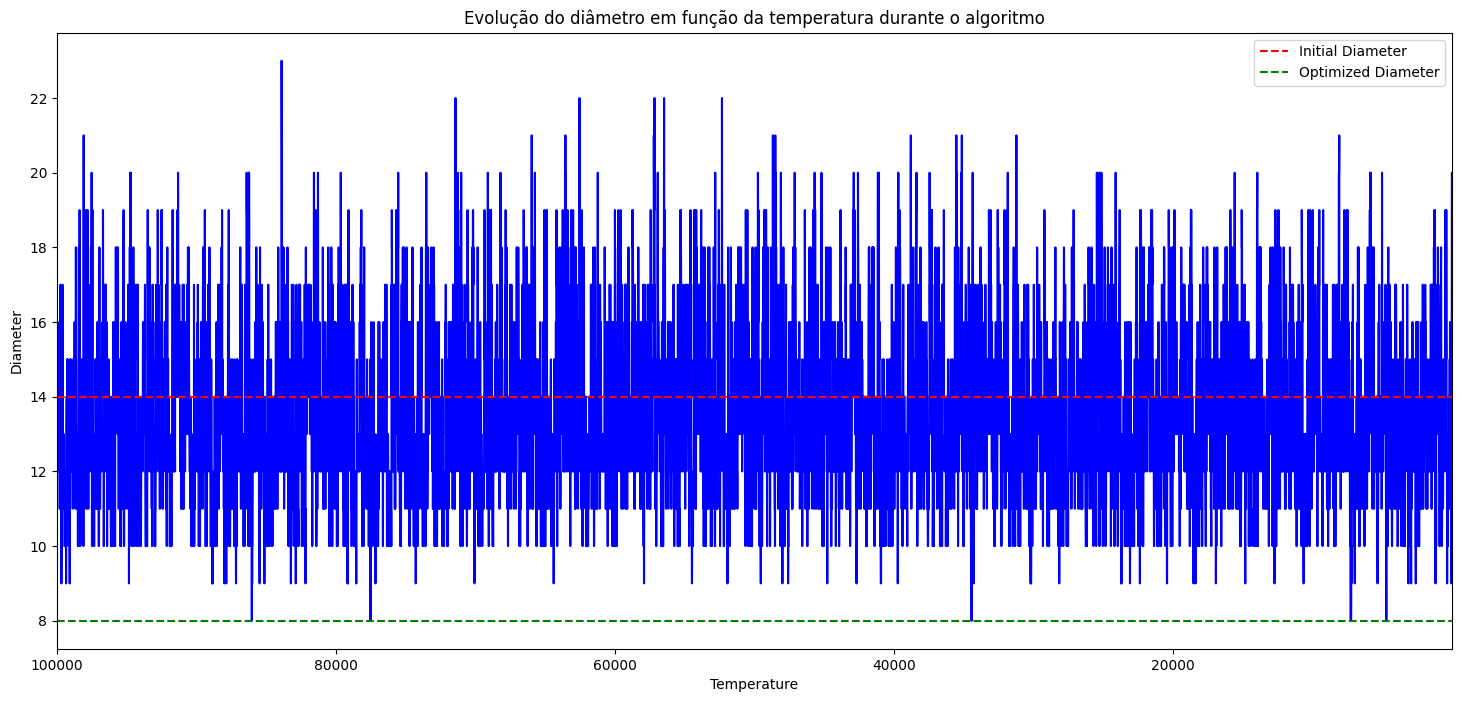
\includegraphics[width = 0.8 \linewidth]{grafic_diameter_13000.png}
        \caption{\small Evolution of diameter}
        \label{fig:diameter}
    \end{figure}
    \begin{figure}[H]
        \centering
        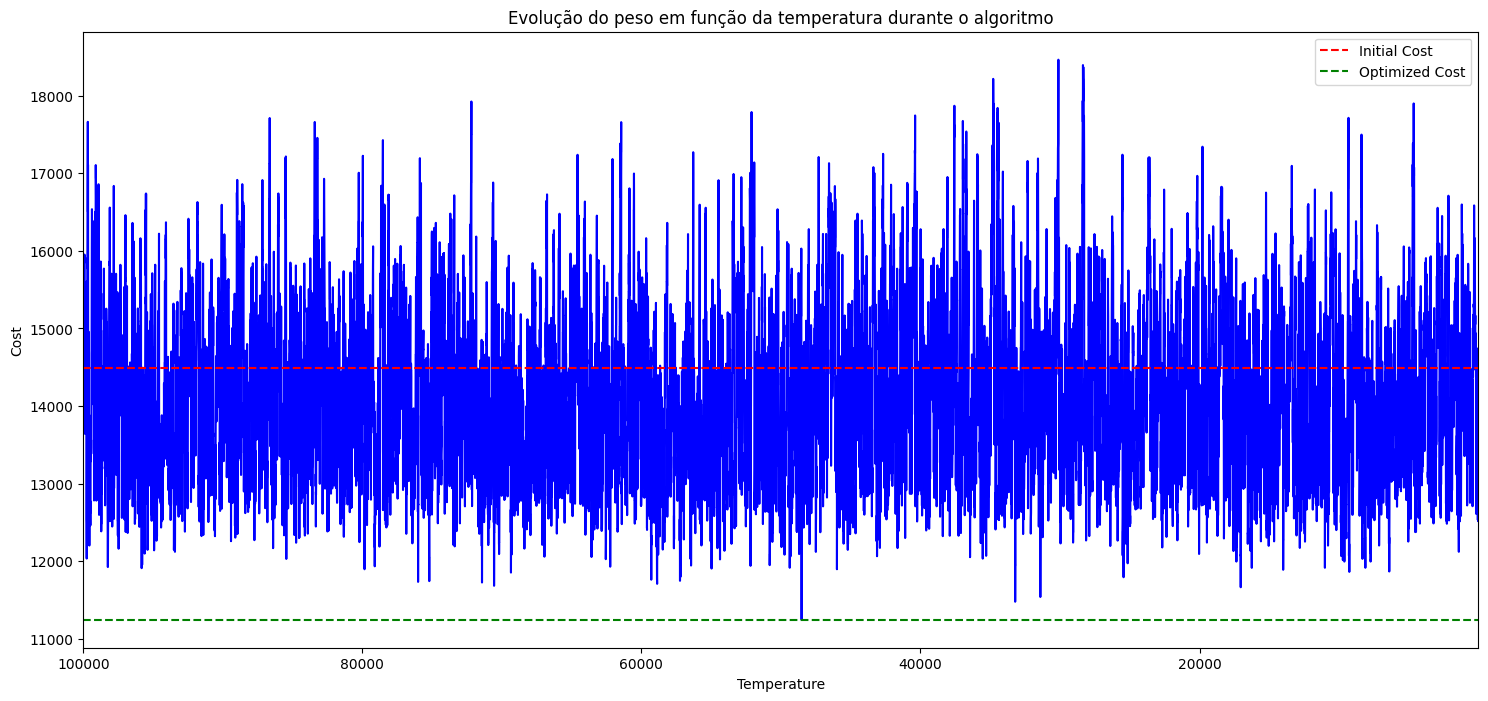
\includegraphics[width = 0.8 \linewidth]{grafic_weight_13000.png}
        \caption{\small Evolution of weight}
        \label{fig:weight}
    \end{figure}
        

\section{Discussion and Conclusion}
Simulated Annealing is an exciting procedure and has much room for improvement. Thus, there are several ways to combine and create parameters, heuristics, and chains. Our work showed a new and exciting perspective of solving the problem. Although it still needs some adjustments to get better, we believe it was an attractive way to deal with the problem. As a result, we got optimality certificate in all tested instances, even with high times. Moreover, it has unique literary importance.

We noticed that the performance was better for instances that are sparse graphs, as expected. In addition, for graphs with many nodes and edges, the algorithm takes longer to converge. For future work, we would like to research better ways to handle transitions. Also, test other cooling strategies and local searches to try to reduce the execution time.

\bibliographystyle{sbc}
\bibliography{sbc-template}

\end{document}
